% =====================================================================
%  Slides de soutenance - Projet "Introduction to Data Processing" (MAM3)
%  Compiler sur OVERLEAF (pdfLaTeX). Uploader tout le dossier "projet fini"
%  et choisir slides/main.tex comme document principal.
% =====================================================================
\documentclass[aspectratio=169]{beamer}
\usetheme{Madrid}
\usecolortheme{whale}
\usepackage[utf8]{inputenc}
\usepackage[T1]{fontenc}
\usepackage[french]{babel}
\usepackage{graphicx}
\usepackage{booktabs}
\graphicspath{{../figures/}{figures/}{./figures/}}
\setbeamertemplate{navigation symbols}{}
\setbeamertemplate{caption}{\raggedright\insertcaption\par}

\title[Prix des voitures d'occasion]{Estimer le prix d'une voiture d'occasion}
\subtitle{Introduction to Data Processing --- MAM3, UCA}
\author{Nathan Barbier \and [Membre 2] \and [Membre 3]}
\date{Juin 2026}

\begin{document}

\begin{frame}\titlepage\end{frame}

% ---------------------------------------------------------------- SLIDE 1
\begin{frame}{1. Problème métier}
  \textbf{Question :} à partir des caractéristiques d'une voiture d'occasion
  (âge, kilométrage, marque, motorisation\dots), peut-on \alert{estimer son prix} ?
  \medskip
  \begin{itemize}
    \item \textbf{Utile} pour : un particulier (vendre/acheter au juste prix),
          un concessionnaire (reprise), un assureur (valeur).
    \item Le prix est une \alert{valeur continue} $\Rightarrow$ problème de
          \textbf{régression} (pas de classification).
    \item \textbf{Dataset :} \emph{100 000 UK Used Cars}, \alert{71\,450 voitures}
          réelles, 7 marques (Audi, BMW, Ford, Hyundai, Skoda, Toyota, VW).
          Données \textbf{antérieures à l'IA générative}.
  \end{itemize}
\end{frame}

% ---------------------------------------------------------------- SLIDE 2
\begin{frame}{2. Les données}
  \begin{columns}
    \begin{column}{0.52\textwidth}
      \footnotesize
      \textbf{10 variables} (1 cible, 6 numériques, 4 catégorielles) :
      \begin{itemize}
        \item \alert{price} (cible), year, mileage, engineSize, tax, mpg
        \item model, Make, transmission, fuelType
      \end{itemize}
      \textbf{Tri / nettoyage :}
      \begin{itemize}
        \item années aberrantes (1970, 2060), doublons, prix/km extrêmes
        \item cylindrée $=0$ \textbf{imputée} (médiane par carburant)
        \item carburants rares regroupés
      \end{itemize}
      Le prix est \alert{très asymétrique} $\Rightarrow$ \texttt{log(prix)} utile.
    \end{column}
    \begin{column}{0.48\textwidth}
      \centering
      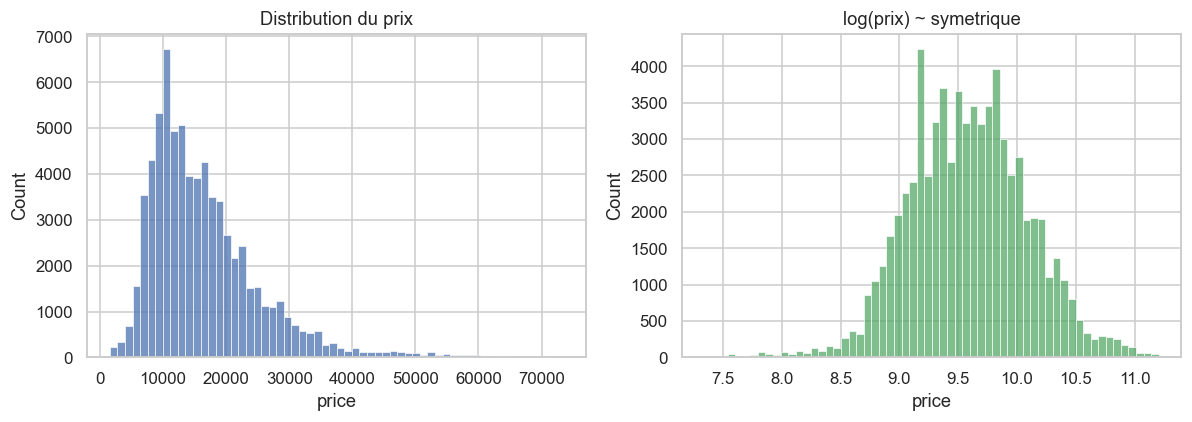
\includegraphics[width=\linewidth]{00_distribution_prix}
    \end{column}
  \end{columns}
\end{frame}

% ---------------------------------------------------------------- SLIDE 3
\begin{frame}{3. Caractéristiques construites (handcrafted features)}
  \begin{columns}
    \begin{column}{0.5\textwidth}
      \footnotesize
      \begin{tabular}{@{}ll@{}}
        \toprule
        Feature & $R^2$ (seule) \\ \midrule
        \texttt{engineSize} & 0.40 \\
        \texttt{car\_age} & 0.28 \\
        \alert{\texttt{log\_mileage}}$^\star$ & \textbf{0.21} \\
        \alert{\texttt{is\_premium}}$^\star$ & 0.19 \\
        \texttt{Odometer} (brut) & 0.19 \\
        \alert{\texttt{age\_x\_mileage}}$^\star$ & 0.15 \\
        \texttt{model} (encodé) & \textbf{0.62} \\ \bottomrule
      \end{tabular}
      \par\medskip
      $\star$ = ajoutées. \texttt{log\_mileage} \alert{bat} le km brut ;
      \texttt{model} encodé (target encoding) est la variable la plus forte.
    \end{column}
    \begin{column}{0.5\textwidth}
      \centering
      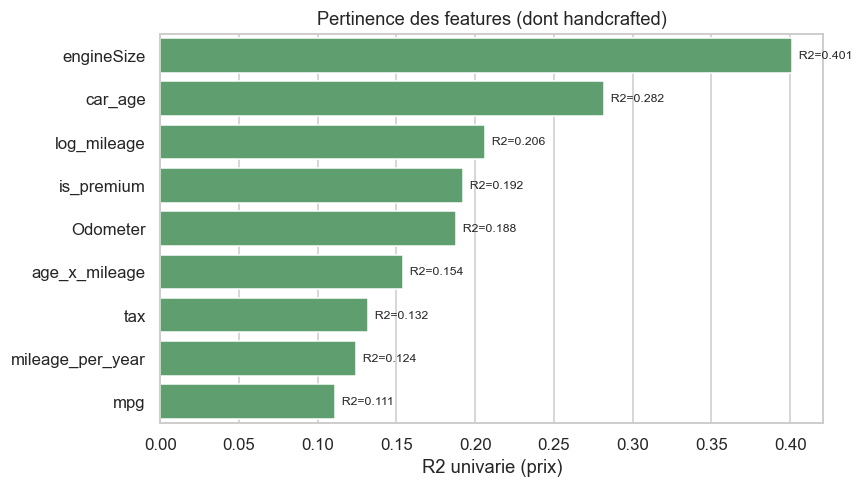
\includegraphics[width=\linewidth]{20_pertinence_features}
    \end{column}
  \end{columns}
\end{frame}

% ---------------------------------------------------------------- SLIDE 4
\begin{frame}{4. Régression : quel modèle ?}
  \textbf{Cible continue $\Rightarrow$ régression linéaire.} Mais le linéaire \alert{brut
  sous-ajuste} (décote exponentielle, km asymétrique). Comparaison en \textbf{validation
  croisée 5 plis} :
  \begin{columns}
    \begin{column}{0.55\textwidth}
      \centering\footnotesize
      % ===MODELES_TABLE_START===
      \begin{tabular}{@{}lcc@{}}
        \toprule
        Modèle & $R^2$ & RMSE \\ \midrule
        Linéaire brut & 0.89 & \pounds2980 \\
        + log(prix) & 0.91 & \pounds2745 \\
        + polynôme & 0.92 & \pounds2541 \\
        \alert{Random Forest} & \alert{0.96} & \alert{\pounds1704} \\
        \bottomrule
      \end{tabular}
      % ===MODELES_TABLE_END===
    \end{column}
    \begin{column}{0.45\textwidth}
      \centering
      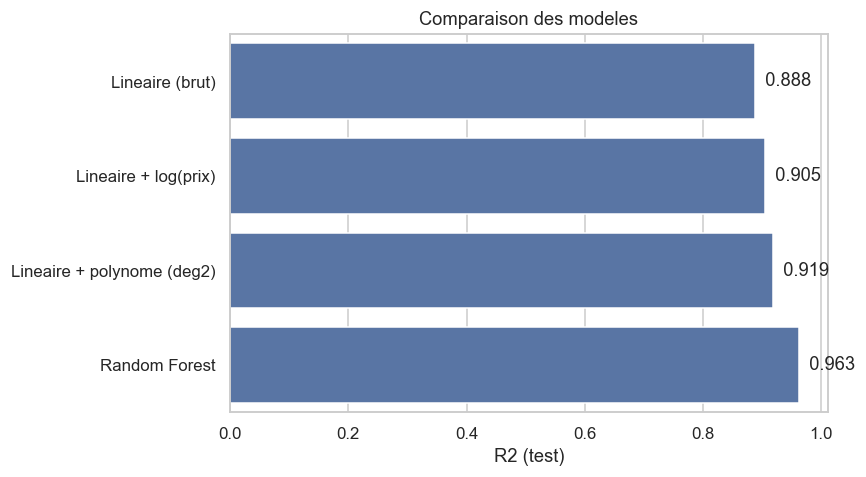
\includegraphics[width=\linewidth]{30_comparaison_modeles}
    \end{column}
  \end{columns}
  \medskip
  {\footnotesize \textbf{Histoire :} prix--âge n'est pas linéaire $\to$ on passe au
  \texttt{log(prix)} / polynôme $\to$ le $R^2$ remonte. Meilleur modèle : \alert{Random Forest ($R^2=0.96$)} ; la linéaire transformée atteint déjà $0.92$.}
\end{frame}

% ---------------------------------------------------------------- SLIDE 5
\begin{frame}{5. Conclusion}
  \begin{itemize}
    \item \textbf{Bénéfice :} on estime le prix et on identifie les facteurs clés
          (\alert{modèle/marque}, âge, cylindrée, kilométrage).
    \item \textbf{La régression linéaire est adaptée} comme modèle \alert{principal et
          interprétable}, \emph{à condition de transformer} (log du prix, features
          polynomiales/log) --- sinon elle sous-ajuste.
    \item \textbf{Peut-on améliorer ?} Oui : modèles non linéaires (\alert{Random Forest},
          Gradient Boosting), réglage des hyperparamètres, plus de marques/features.
          Compromis \textbf{performance $\leftrightarrow$ interprétabilité}.
    \item \textbf{Limites :} marché UK (prix en £), features non exhaustives.
  \end{itemize}
  \vfill
  \centering\small Merci ! \quad Questions ?
\end{frame}

\end{document}
